\chapter{Tolman-Oppenheimer-Volkoff equation}
\label{chap:tov}

In 1687, Sir Isaac Newton sparked a revolution in the field of physics when he described motion of bodies with the concept of forces and modeled gravity as an attractive force
\cite{ref:newton}
\begin{equation*}
	\vec{F} = - G \frac{m_1 m_2}{r^2} \vec{\hat{r}} .
\end{equation*}
For a long time, his three laws of motion and law of gravity seemed to accurately explain all observable macroscopic motion.
In particular, his laws provided an explanation for the three laws of planetary motion that Johannes Kepler found by empirical observation many years earlier in 1609 \cite{ref:kepler1} and 1619 \cite{ref:kepler2}.

However, in 1859, Urbain Le Verrier observed that Mercury's orbit deviates from the one predicted by Kepler's and Newton's laws \cite{ref:le_verrier}.
The resolution came half a century later, when Albert Einstein proposed his theory of special relativity in 1905 \cite{ref:einstein_special} and ten years later incorporated gravity into this framework with the theory of general relativity \cite{ref:einstein_general}.
%Newton: gravity affects body, body does not move along straight path
%Einstein: gravity affects space, body moves along straight path
While Newton thought gravity \emph{disturbs a body} from moving straight through spacetime, Einstein explained gravity as \emph{curvature of spacetime} that instead reshapes the straight paths along which a body moves.
Such a ``curved straight path'' is called a \emph{geodesic}.
%While Newton thought gravity affects a body and disturbs its straight motion through flat space, Einstein instead thought gravity \emph{curves} space and thus changes the straight paths along which bodies move.
%Instead of describing gravity as a force that disturbs straight motion through flat space, Einstein argued that gravity rather \emph{curves} space and time and thus alters the paths along which straight motion occurs.
%Instead of describing gravity as a force that disturbs straight motion through flat space, Einstein explained that gravity \emph{curves} space and time and alters the paths along which straight motion occurs.
%Einstein argued that bodies \emph{do} move along straight paths through space and time that have been \emph{curved} by the presence of mass and energy according to the Einstein field equations
Spacetime is curved according to the Einstein field equations
\begin{equation*}
	G\indices{_\mu_\nu} = R_{\mu \nu} - \frac{1}{2} R g_{\mu \nu} = \frac{8 \pi G}{c^4} T_{\mu \nu} ,
\end{equation*}
expressing how energy and momentum on the rightmost side -- such as mass and light -- determine the geometry of spacetime on the left side.

The most important result of this chapter will be the Tolman-Oppenheimer-Volkoff equation
\begin{equation*}
	\odv{P(r)}{r} = -\frac{G m(r) \epsilon(r)}{r^2 c^2} \left[ 1 + \frac{P(r)}{\epsilon(r)} \right] \left[ 1 + \frac{4 \pi r^3 P(r)}{m(r) c^2} \right] \left[ 1 - \frac{2 G m(r)}{r c^2} \right]^{-1} ,
\end{equation*}
which we will derive from the Einstein field equations.
With this equation, we can find the pressure profile and radius of a star once we have an equation of state that relates the pressure and energy of the material inside.
This will be an essential tool for our following analysis of different equations of state.
The equation was originally derived in 1939 by Robert Oppenheimer and George Volkoff \cite{ref:tov}, building on earlier work of Richard Tolman \cite{ref:tolman}.

We will also examine the general consequences of this equation applied to the extreme case of an incompressible star. 
To make sense of our results, we will investigate the correspondence between general relativity and Newtonian gravity in the limit of small velocoties and weak gravitational fields.

\textit{This chapter is inspired by references \cite{ref:carroll}, \cite{ref:mtw} and \cite{ref:mika_gr_notes}.}

\section{Derivation from the Einstein field equations}
\label{sec:einstein_to_tov}

To analyze astrophysical objects like stars, it is of considerable interest to relate the pressure $P(x)$ and energy density $\epsilon(x)$ or mass density $\rho(x)$ at every position $x$ inside the object.
We will derive the relativistic relation between these quantities from the \textbf{Einstein field equations} \cite[equation 4.44]{ref:carroll}
\begin{equation}
	G\indices{_\mu_\nu} = R_{\mu \nu} - \frac{1}{2} R g_{\mu \nu} = \frac{8 \pi G}{c^4} T_{\mu \nu} .
	\label{eq:einstein}
\end{equation}
It describes how the geometry of spacetime, described by the Ricci tensor $R\indices{_\mu_\nu}$ and Ricci scalar $R$ that are ultimately built from the metric $g\indices{_\mu_\nu}$ and encapsulated in the Einstein tensor $G\indices{_\mu_\nu}$ (see \cref{chap:gr_summary} for a summary), responds to the presence of energy-momentum in the energy-momentum tensor $T\indices{_\mu_\nu}$.
Here, $G$ is the gravitational constant and $c$ is the speed of light.
As we later compare our findings to those of Newtonian gravity, it will be useful to connect the energy density to the mass density by the \textbf{mass-energy equivalence relation}
\begin{equation}
	\epsilon(x) = \rho(x) c^2 .
	\label{eq:tov:mass_energy_equivalence}
\end{equation}

Unless rotating very fast, stars are well approximated by spheres.
For our purposes, we therefore use the coordinates
\begin{equation}
	x^\mu = (c t, r, \theta, \phi)
	\quad \text{with} \quad
	-\infty < t < \infty, \quad
	0 \leq r < \infty, \quad
	0 \leq \theta \leq \pi, \quad
	0 \leq \phi < 2 \pi .
\end{equation}
and consider the most general metric that exhibits spherical symmetry, \cite[equation 5.11]{ref:carroll}
\begin{equation}
	% coordinates x = (ct, r, θ, ϕ)
	\dif s^2 = e^{2 \alpha(r)} c^2 \dif t^2 - e^{2 \beta(r)} \dif r^2 - r^2 \left( \dif \theta^2 + \sin^2 \theta \dif \phi^2 \right) .
\label{eq:tov:metric}
\end{equation}

We model the interior of the star as a perfect fluid in equilibrium.
In \cref{chap:relfluid}, we show that a perfect fluid has the energy-momentum tensor
\begin{equation}
	T\indices{_\mu_\nu}(r) = \frac{u_\mu u_\nu}{c^2} \left[ \epsilon(r)+P(r) \right]  - g\indices{_\mu_\nu} P(r) .
	\label{eq:tov:energy_momentum_perfect_fluid}
\end{equation}
The analysis is simplest in the rest frame of the fluid, where $u_\mu = (u_0, \textbf{0})$ and the normalization condition $u_\mu u^\mu = c^2$ requires $u_0 = \pm e^\alpha c$.
We choose the positive sign so the four-velocity lies in the future light cone, as we are interested in the evolution of the star.
Dropping the function argument $r$ from now, the energy-momentum tensor then takes the diagonal form
\begin{equation}
T\indices{_\mu_\nu} =
\begin{bmatrix}
	\epsilon e^{2\alpha} & 0            & 0     & 0                   \\
	0                    & P e^{2\beta} & 0     & 0                   \\
	0                    & 0            & P r^2 & 0                   \\
	0                    & 0            & 0     & P r^2 \sin^2 \theta \\
\end{bmatrix}
\qquad \text{or} \qquad
T\indices{_\mu^\nu} =
\begin{bmatrix}
	\epsilon &  0 &  0 &  0 \\
	0        & -P &  0 &  0 \\
	0        &  0 & -P &  0 \\
	0        &  0 &  0 & -P \\
\end{bmatrix}
.
\label{eq:einstein_to_tov:T}
\end{equation}

Starting with the metric, it is now straightforward, although tedious, to compute the left side of \cref{eq:einstein} from \cref{eq:def_christoffel,eq:def_riemann_tensor,eq:def_ricci_tensor,eq:def_ricci_scalar}.
For the details, refer to \cite[equation 5.11-5.15]{ref:carroll} or \cref{sec:tov_cas_derivation}.
After inserting the energy-momentum tensor on the right and simplifying, we get the three independent equations
(the fourth turns out proportional to the third)
\begin{subequations}
\begin{align}
	\frac{1}{r^2} e^{-2 \beta} \left( 2 r \beta' - 1 + e^{2 \beta} \right)                               &= \frac{8 \pi G}{c^4} \epsilon
	&& \left( G\indices{_0_0} = \frac{8 \pi G}{c^4} T\indices{_0_0} \right) , \label{eq:einstein_to_tov:tt} \\
	\frac{1}{r^2} e^{-2 \beta} \left( 2 r \alpha' + 1 - e^{2 \beta} \right)                              &= \frac{8 \pi G}{c^4} P
	&& \left( G\indices{_1_1} = \frac{8 \pi G}{c^4} T\indices{_1_1} \right) , \label{eq:einstein_to_tov:rr} \\
	e^{-2 \beta} \left( \alpha'' + (\alpha')^2 - \alpha' \beta' + \frac{1}{r} (\alpha' - \beta') \right) &= \frac{8 \pi G}{c^4} P
	&& \left( G\indices{_2_2} = \frac{8 \pi G}{c^4} T\indices{_2_2} \right) . \label{eq:einstein_to_tov:thetatheta}
\end{align}
\label{eq:einstein_to_tov:einstein_equation_in_star}
\end{subequations}

\subsubsection{Exterior solution}

First, let us quickly review the Schwarzschild solution outside the star, where there is no pressure nor energy density and all right sides vanish.
Adding equation \eqref{eq:einstein_to_tov:tt} and \eqref{eq:einstein_to_tov:rr} then yields $(\alpha + \beta)' = 0$, so $\alpha + \beta = C$ for some constant $C$.
The constant can be found by noting that far away from the star, as $r \rightarrow \infty$, the metric should reduce to the Minkowski metric with $e^{2\alpha} = e^{2 \beta} = 1$, so we must have $\alpha + \beta = 0$.
Inserting $\beta' = -\alpha'$ into equation \eqref{eq:einstein_to_tov:thetatheta} then gives a differential equation for $\alpha$ whose solution is $\alpha = \log \left( 1 - D / r \right) / 2$ for some constant $D$.
To determine it, we use that in the Newtonian limit \eqref{eq:weak_field_limit:metric_with_potential}, the temporal metric element should reduce to $e^{2 \alpha} = 1 + 2 V / c^2$ where $V = - G M / r$ is the Newtonian gravitational potential of the star and $M$ is the \emph{Newtonian mass} of the star.
Thus, the metric outside the star is the well-known \textbf{Schwarzschild metric}
\begin{equation}
	\dif s^2 = \left( 1 - \frac{2 G M}{r c^2} \right) c^2 \dif t^2 - \left( 1 - \frac{2 G M}{r c^2} \right)^{-1} \dif r^2 - r^2 \left( \dif \theta^2 + \sin^2 \theta \dif \phi^2 \right) .
\label{eq:tov:schwarzschild_metric}
\end{equation}
Observe that the metric is singular at the \textbf{Schwarzschild radius}
\begin{equation}
	r = R_S = 2 G M / c^2.
\label{eq:tov:schwarzschild_radius}
\end{equation}
This is an \emph{event horizon}, from which not even light can escape out of. \cite[section 5.6]{ref:carroll}.
If a star is so small and massive that its Schwarzschild radius $R_S > R$ lies \emph{outside} the surface, the star is invisible from the outside and we say it has collapsed to a \textbf{black hole}.

\subsubsection{Interior solution}

We now return to the analysis inside the star.
To imitate the Schwarzschild metric element $g_{11}$, let us define the function $m(r)$ by
\begin{equation}
	e^{2 \beta(r)} = \left[ 1 - \frac{2 G m(r)}{r c^2} \right]^{-1} .
	\label{eq:einstein_to_tov:def_m}
\end{equation}
Then \cref{eq:einstein_to_tov:tt} becomes
\begin{equation}
	\odv{\left[m(r) c^2\right]}{r} = 4 \pi r^2 \epsilon(r) ,
	\label{eq:einstein_to_tov:m_rho}
\end{equation}
directly relating $m(r)$ and $\epsilon(r)$.
If we set $m(0) = 0$, we can integrate to get
\begin{equation}
	m(r) c^2 = \integral{\epsilon(r') 4 \pi r'^2}{r'}{0}{r} .
	\label{eq:einstein_to_tov:m_integral}
\end{equation}
In \cite[page 602]{ref:mtw} it is shown that setting $m(0) \neq 0$ creates a singularity at the origin, which is not physically acceptable.
Meanwhile, definition \eqref{eq:einstein_to_tov:def_m} turns \cref{eq:einstein_to_tov:rr} into
\begin{equation}
	\odv{\alpha(r)}{r} = \frac{G}{r^2 c^4} \frac{m(r) c^2 + 4 \pi r^3 P(r)}{1 - 2 G m(r) / r c^2} .
	\label{eq:einstein_to_tov:dadr1}
\end{equation}
To finally eliminate $\alpha$, we can replace all occurences of $\alpha'$ and $\beta$ in the remaining \cref{eq:einstein_to_tov:thetatheta} with the expressions \eqref{eq:einstein_to_tov:dadr1} and \eqref{eq:einstein_to_tov:def_m}.
Doing so is straightforward, but cumbersome and most easily done by a computer algebra system.
We show how to do this in \cref{sec:tov_cas_derivation}.
An elegant, but less straightforward argument is to use local energy-momentum conservation $\nabla_\mu T\indices{^\mu^\nu} = 0$, which is both physically reasonable and in fact possible to prove directly from the Einstein field equations \eqref{eq:einstein}.
For two different proofs, see \cite{ref:einstein_conservation_energy_momentum} and \cite[section 8.3.2]{ref:mika_gr_notes}.
Using \cref{eq:def_cov_deriv}, the component $\nu=1$ gives
\begin{equation*}
\begin{split}
	0 &= \nabla_\mu T\indices{^\mu_1} \\
	  &= \partial_1 T\indices{^1_1} + \Gamma^\sigma_{1 \sigma} T\indices{^1_1} - \Gamma^\sigma_{1 \mu} T\indices{^\mu_\sigma} \\
	  &= \partial_1 T\indices{^1_1} + \Gamma^0_{10} T\indices{^1_1} + \sum_{i=1}^3 \Gamma^i_{1i} T\indices{^1_1} - \Gamma^0_{10} T\indices{^0_0} - \sum_{i=1}^3 \Gamma^i_{1i} T\indices{^i_i} . \\
\end{split}
\end{equation*}
Using $T\indices{^0_0} = \epsilon$ and $T\indices{^1_1} = T\indices{^2_2} = T\indices{^3_3} = -P$ from \cref{eq:einstein_to_tov:T}, the explicit sums cancel.
With $\Gamma^0_{10} = \frac12 g^{00} \partial_1 g_{00} = \odv{\alpha}/{r}$, we are left with
\begin{equation}
	\odv{\alpha}{r} = \frac{-1}{\epsilon+P} \odv{P}{r} .
	\label{eq:einstein_to_tov:dadr2}
\end{equation}
Now $\alpha$ is easily eliminated by equating \eqref{eq:einstein_to_tov:dadr1} and \eqref{eq:einstein_to_tov:dadr2}. 
Whichever approach we follow, we end up with the \textbf{Tolman-Oppenheimer-Volkoff (TOV) equation}
\begin{equation}
	\odv{P(r)}{r} = -\frac{G m(r) \epsilon(r)}{r^2 c^2} \left[ 1 + \frac{P(r)}{\epsilon(r)} \right] \left[ 1 + \frac{4 \pi r^3 P(r)}{m(r) c^2} \right] \left[ 1 - \frac{2 G m(r)}{r c^2} \right]^{-1} .
	\label{eq:tov}
\end{equation}
It relates the pressure gradient $\odv{P}/{r}$ and energy density $\epsilon$ at radius $r$ from the center of a spherical static star composed of a perfect fluid.
\Cref{eq:einstein_to_tov:m_rho,eq:tov} constitute two equations for the three unknowns $P$, $\epsilon$ and $m$.
To determine them, an additional \textbf{equation of state}
\begin{equation}
	\epsilon = \epsilon(P)
\label{eq:tov:eos}
\end{equation}
that relates the thermodynamic variables is required, typically obtained from statistical physics.
Given all three equations \eqref{eq:einstein_to_tov:m_rho}, \eqref{eq:tov} and \eqref{eq:tov:eos}, the initial mass $m(0) = 0$ and some central pressure $P(0) = P_c$ or energy density $\epsilon(0) = \epsilon_c$, we can integrate them to find the pressure $P(r)$, mass $m(r)$ and energy density $\epsilon(r)$ everywhere inside the star.
We define the surface of the star to be the radius $r=R$ at which $P(r) = 0$, and the star's mass as the corresponding value $m(R) = M$.
If desired, we can then calculate the metric function $\beta(r)$ from definition \eqref{eq:einstein_to_tov:def_m}, and $\alpha(r)$ by integrating \cref{eq:einstein_to_tov:dadr2} from the surface $r=R$, where it must match the Schwarzschild metric \eqref{eq:tov:schwarzschild_metric}, and back into the center $r=0$.
Solving these equations is therefore our ultimate goal.

\iffalse
For some purposes, such as when analyzing stability of stars in \cref{sec:nstars:stability_general}, it is also useful to obtain the metric function $\alpha(r)$.
Inside the star, note that in both equation \eqref{eq:einstein_to_tov:einstein_equation_in_star} and \eqref{eq:einstein_to_tov:dadr2}, it is only the derivative $\alpha'(r)$ that enters, so the solution is only specified up to a constant.
Outside the star, however, $\alpha(R)$ should match the Schwarzschild metric with
\begin{equation}
	g_{00} = e^{2 \alpha(R)} = 1 - \frac{2 G M }{Rc^2} .
\label{eq:tov:schwarzschild_metric_00_surface}
\end{equation}
To integrate $\alpha(r)$, then, we can simply start with any value such as $\alpha(0) = 0$ at the center, then integrate either \eqref{eq:einstein_to_tov:dadr1} or \eqref{eq:einstein_to_tov:dadr2} with the \emph{known} right sides out to the surface $r=R$ and finally shift all values of $\alpha(r)$ by
\begin{equation}
	\alpha(r) \rightarrow \alpha(r) - \alpha(R) + \frac12 \log \left( 1 - \frac{2 G M }{ R c^2} \right)
\end{equation}
to match the Schwarzschild metric element \eqref{eq:tov:schwarzschild_metric_00_surface}.
This is completely equivalent to instead setting $\alpha(R) = \log \left(1 - 2 G M / R c^2 \right) / 2$ and integrating $\odv{\alpha(r)}/{r}$ backwards from the surface $r=R$ into the center $r=0$, but the former method can be more natural to implement from a numerical perspective.
\fi

\subsubsection{Interpretation of mass}

One matter that deserves comment is our definition of the star's mass $M = m(R)$.
We should be a little careful about this, since it is not obvious how to think of ``mass'' in relativistic terms.
At the surface $r=R$ of the star, our metric must match the Schwarzschild metric \eqref{eq:tov:schwarzschild_metric}.
Comparing the definition \eqref{eq:einstein_to_tov:def_m} of $m(r)$ to the Schwarzschild metric, we then see that
\begin{equation}
	m(R) = M = \frac{1}{c^2} \integral{\epsilon(r) 4 \pi r^2}{r}{0}{R} = \integral{\rho(r) 4 \pi r^2}{r}{0}{R}
	\label{eq:einstein_to_tov:schwarzschild_mass}
\end{equation}
is the same mass that appears in the Schwarzschild metric, which we \emph{defined} to be the \emph{Newtonian mass} of the star.
However, the factor $4 \pi r^2$ in the integral is not a proper volume element, as it is missing the factor $e^{\beta(r)}$ from the full spatial metric determinant.
The true volume integral of the star's energy density is really
\begin{equation*}
	\bar{M} c^2 = \integral{\epsilon(r) e^{\beta(r)} 4 \pi r^2}{r}{0}{R} .
\end{equation*}
In fact, the difference
\begin{equation*}
	\bar{M} c^2 - M c^2 = \integral{\epsilon(r) \left[ \left( 1-\frac{2Gm(r)}{rc^2} \right)^{-1/2} - 1 \right] 4 \pi r^2}{r}{0}{R} > 0
\end{equation*}
is the binding energy that arises due to the gravitational attraction between the individual fluid elements in the star.
To see this, take the Newtonian limit \eqref{eq:weak_field_limit:weak_field_metric} of the element $g_{00}$ of the Schwarzschild metric \eqref{eq:tov:schwarzschild_metric} to see that we have the small quantity
\begin{equation}
	\frac{G m(r)}{rc^2} \ll 1 .
	\label{eq:weak_field_limit:small_gmr}
\end{equation}
Using the Taylor expansion $(1 - x)^{-1/2} = 1 + x/2$ and the mass-energy equivalence relation \eqref{eq:tov:mass_energy_equivalence}, we then get
\begin{equation}
	\bar{M} c^2 - M c^2 \taylor \integral{\frac{\epsilon(r)}{c^2} \frac{GM}{r} 4 \pi r^2}{r}{0}{R}
	                    =       \integral{\rho(r) \frac{GM}{r} 4 \pi r^2}{r}{0}{R} .
\end{equation}
As shown in \cite[exercise 23.7]{ref:mtw}, this is precisely the energy required to construct the star by sequentially placing thin shells of mass $\dif m = \rho(r) 4 \pi r^2 \dif r$ on top of each other, each subject to the gravitational attraction of the shells already placed below it.
This explains that $\bar{M} c^2 - M c^2$ is indeed the binding energy that would be required to disperse all the matter in the star to infinity.

The moral of this story is that the mass $M = m(R)$ in the Tolman-Oppenheimer-Volkoff equation should be interpreted as the \emph{Newtonian} mass of the star.
But $M c^2$ is \emph{not} the total energy of the star, as we saw above that it differs by the binding energy.
Experimentally, this implies that we can measure masses of distant stars using \emph{Newtonian} results like Kepler's third law \cite[chapter 19]{ref:mtw} that rely only on simple observations.
Moreover, it makes it meaningful to compare masses obtained from general relativity to those found using Newtonian gravity.
% confusion about M, \bar{M}, resources:
% https://physics.stackexchange.com/q/196280/299916
% see MTW p. 602-, box at p. 603, p. 453
% see Schwarz p. 126
\section{Solution for an incompressible star}
\label{sec:incompressible_star}

% TODO: an incompressible star is unphysical

Although it may sound unphysical from the outset, we can make a somewhat realistic model of a star by assuming that the fluid is incompressible, meaning the energy density
\begin{equation}
	\epsilon(r) = \epsilon_0
\end{equation}
is constant inside the star.
For example, the speed of sound \eqref{eq:relfluid:speed_of_sound} takes the completely unrealistic value $v = c \sqrt{\odv{P}/{\epsilon}} = c \sqrt{1/(\odv{\epsilon}/{P})} = c \sqrt{1/0} = \infty$.
Anyway, integrating \cref{eq:einstein_to_tov:m_integral,eq:einstein_to_tov:schwarzschild_mass} yield
\begin{equation}
	m(r) c^2 = \frac{4}{3} \pi r^3 \epsilon_0 
	\quad \text{and} \quad
	M c^2 = \frac{4}{3} \pi R^3 \epsilon_0 
	.
\end{equation}
Inserting the energy density $\epsilon(r)$ and mass $m(r)$ into \cref{eq:tov}, $P$ and $r$ separate to
\begin{equation*}
	\int \frac{\dif P}{(\epsilon_0+P)(\epsilon_0+3P)} = - \int \frac{4 \pi G r \dif r}{3 c^4 - 8\pi G r^2 \epsilon_0} .
\end{equation*}
The left side can now be split by the partial fraction decomposition
\begin{equation*}
	\frac{1}{(\epsilon_0+P)(\epsilon_0+3P)} = \frac{1}{2P} \left( \frac{1}{\epsilon_0+P} + \frac{1}{\epsilon_0+3P} \right) .
\end{equation*}
Applying integral \eqref{eq:integrals:logarithm_xnum} and \eqref{eq:integrals:logarithm_1num} and imposing the boundary condition $P(R) = 0$, we eventually find the pressure
\begin{equation}
	% p(r) in terms of M, R, 
	P(r) = \epsilon_0 \, \frac{\sqrt{1-\frac{2GMr^2}{R^3c^2}} - \sqrt{1-\frac{2GM}{Rc^2}}}{3 \sqrt{1-\frac{2GM}{Rc^2}} - \sqrt{1-\frac{2GMr^2}{R^3c^2}}} .
	% p(r) in terms of p0, M, R
	%p(r) = -\frac{M}{\frac{4}{3} \pi R^3} \frac{4 \pi R^{3} p_0 \left( \frac{1}{3} + \sqrt{1-\frac{2GMr^2}{R^3}} \right) + M \left( 1 + \sqrt{1-\frac{2GMr^2}{R^3}} \right)}
	%                                           {4 \pi R^{3} p_0 \left( 1           + \sqrt{1-\frac{2GMr^2}{R^3}} \right) + M \left( 3 + \sqrt{1-\frac{2GMr^2}{R^3}} \right)}
	\label{eq:incompressible_star:pressure}
\end{equation}
In particular, the central pressure is
\begin{equation}
	P(0) = \epsilon_0 \frac{1 - \sqrt{1 - \frac{2GM}{Rc^2}}}{3 \sqrt{1-\frac{2GM}{Rc^2}} - 1} .
	\label{eq:incompressible_star:central_pressure}
\end{equation}
It is interesting to note that the pressure is positive for $GM/Rc^2 < 4/9$, but explodes at $GM/Rc^2 = 4/9$ and becomes negative for $GM/Rc^2 > 4/9$.
The pressure profile of stars approaching this limit is shown in \cref{fig:incompressible_star:plot2}.
Physically, this means that any star compressed to this limit could only be supported by an unattainable infinite central pressure, so it would have no other choice than to collapse.
This is an example of a more general result -- \textbf{Buchdal's theorem} states that all static spherical stars composed of perfect fluids must have
\begin{equation}
	M(R) < M_\text{max}(R) = \frac{4c^2}{9G} R
	\label{eq:incompressible_star:buchdal}
\end{equation}
for any energy density profile $\epsilon(r)$ that does not decrease outwards \cite{ref:buchdal}.
The proof requires careful work, but we can still understand the result intuitively.
If there is a maximum density that is supported by nature, then the most massive object we can make would necessarily have that density everywhere.
Thus, the bound we have found in our computation with constant energy density should be the most extreme bound.
In \cref{fig:incompressible_star:plot1}, we compare the mass-radius relation to this maximum supported mass.

% Ideal use of groupplot + subcaption:
% * use title={\subcaption{...}} for subcaptions (https://tex.stackexchange.com/a/310403)
% * set title style text width automatically (https://tex.stackexchange.com/a/276214)
% * another example (https://tex.stackexchange.com/a/69729)
\begin{figure}[t]
	\centering
	\begin{tikzpicture}[declare function={
		G = 1;
		M(\R,\E) = 4/3*pi*(\R)^3*\E;
		Mmax(\R) = 4*\R/(9*G);
		p(\r,\M,\R) = \M / (4/3*pi*(\R)^3) * (sqrt(1-2*G*\M*(\r)^2/(\R)^3) - sqrt(1-2*G*\M/(\R))) / (3*sqrt(1-2*G*\M/(\R)) - sqrt(1-2*G*\M*(\r)^2/(\R)^3));
	}]
		\begin{groupplot}[group style={group size=2 by 1, horizontal sep=0.1\textwidth}, width=0.49\textwidth]
		\nextgroupplot[
			title={\subcaption{\label{fig:incompressible_star:plot1}Mass-radius relation}},
			xlabel=$R \, / \, R_0$, ylabel=$M(R) \, / \, M(R_0)$, xtick distance=1, 
			legend pos=north west, legend cell align=left,
		]
		\pgfplotsinvokeforeach{0.006} {
			\addplot [domain=0:5, solid ] {M(x,#1) / M(1,#1)}; % node[pos=0.90, sloped, yshift=+6pt] {\scriptsize $\epsilon_0 = #1$};
			\addplot [domain=0:5, dashed] {Mmax(x) / M(1,#1)}; % node[pos=0.2, pin=above:{$M_\text{max}(R)$}] {};
		}
		\legend{$M(R)$, $M_\text{max}(R)$};
		\nextgroupplot[
			title={\subcaption{\label{fig:incompressible_star:plot2}Pressure profile}},
			xlabel=$r\, /\, R_0$, ylabel=$P(r) \, / \, P(0)$, xtick distance=0.25,
		]
		\pgfplotsinvokeforeach{0.9, 0.99, 0.999} {
			\addplot [domain=0:1,samples=200] {p(x,#1*Mmax(1),1)/p(0,#1*Mmax(1),1)} node[pos=0.54, sloped, yshift=+16pt] {\scriptsize $M = #1 M_\text{max}$};
		}
		\end{groupplot}
	\end{tikzpicture}
	\caption{
		\subref{fig:incompressible_star:plot1} Mass-radius relation $M(R) = 4 \pi R^3 \epsilon_0 / 3 c^2$ for a star of constant energy density $\epsilon_0$ compared to the maximum supported mass $M_\text{max}(R) = 4 c^2 R / 9 G$.
		\subref{fig:incompressible_star:plot2} Pressure profile $P(r)$ for stars of radius $R_0 = \sqrt{c^4 / G \epsilon_0}$ and masses $M$ approaching the limit $M_\text{max}(R_0)$.
	}
\end{figure}

Another way of looking at the Buchdal's theorem is that the radius of a star must satisfy
\begin{equation}
	R > \frac94 \frac{G M}{c^2} = \frac98 R_S ,
\end{equation}
where $R_S$ is the Schwarzschild radius \eqref{eq:tov:schwarzschild_radius}.
Since $R > 9 R_S / 8 > R_S$, we see that a stable star that satisfies the Buchdal bound $R > 9 G M / 4 c^2$ is guaranteed to not be a black hole.
If we somehow \emph{do} manage to compress a star to the radius $R = 9 R_S / 8$, we expect it would become unstable, implode and collapse further until its surface is inside the Schwarzschild radius, hence becoming a black hole.

We will shortly see that Buchdal's theorem is a relativistic result and that no such bound arises from Newtonian gravity.

\section{Newtonian limit}

In \cref{sec:weak_field_limit}, we thorougly discuss the conditions under which one should expect general relativity to reduce to Newtonian gravity.
Let us derive the pressure gradient in a star using Newtonian gravity and show that the Tolman-Oppenheimer-Volkoff equation \eqref{eq:tov} reduces to it in the Newtonian limit.

\begin{figure}
\centering
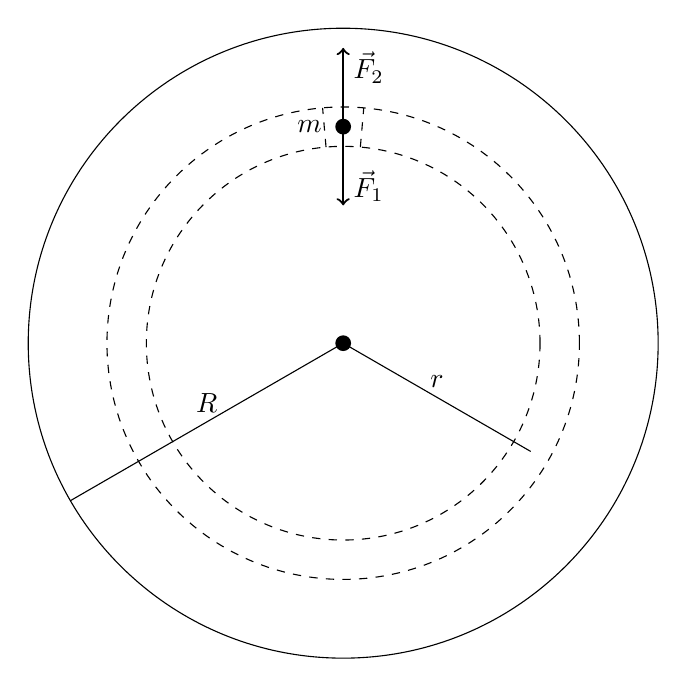
\begin{tikzpicture}
\draw[dashed] (85:2.5) -- (85:3.0);
\draw[dashed] (95:2.5) -- (95:3.0);
\draw [->, thick] (90:2.75) -- (90:1.75) node [near end, right] {$\dif \vec{F}_1$};
\draw [->, thick] (90:2.75) -- (90:3.75) node [near end, right] {$\dif \vec{F}_2$};
\fill (90:2.75) circle [radius=0.1cm];
\node[left=0.15cm] at (90:2.75) {$\dif m$};
\draw[dashed] (0,0) circle [radius=3cm];
\draw[dashed] (0,0) circle [radius=2.5cm];
\draw (0,0) circle [radius=4.0cm];
\fill (0,0) circle [radius=0.1cm];
\draw (0,0) -- (-30:2.75) node [midway,above] {$r$};
\draw (0,0) -- (210:4.0) node [midway,above] {$R$};
\end{tikzpicture}
\caption{\label{fig:hydrostatic_equilibrium_sphere}When a star of radius $R$ is in hydrostatic equilibrium, the gravitational force $\dif \vec{F}_1$ acting on a mass element  $\dif m$ at distance $r$ from the center must exactly cancel the pressure gradient force $\dif \vec{F}_2$.}
\end{figure}

Following \cref{fig:hydrostatic_equilibrium_sphere}, consider the mass element $\dif m = \rho(r) \dif A \dif r$ at distance $r$ from the center of a Newtonian star.
By Gauss' law it is attracted to the mass $m(r)$ inside the radius $r$ as if it were concentrated at the center, but experiences no attraction whatsoever from the remaining mass outside $r$ due to symmetry.
By Newton's law of gravity it is therefore pulled upon by the force
\begin{equation}
	\dif \mathbf{F}_1 = -\frac{G m(r) \dif m}{r^2} \hat{\textbf{r}} .
	\label{eq:weak_field_limit:force_newton}
\end{equation}
If the star is in hydrostatic equilibrium, this force must be exactly cancelled by the force
\begin{equation}
	\dif \textbf{F}_2 = - \Big[ P(r + \dif r) - P(r) \Big] \dif A \, \hat{\textbf{r}} = -\dif P \dif A \, \hat{\textbf{r}}
	\label{eq:weak_field_limit:force_pressure}
\end{equation}
that arises from the pressure difference above and below the element.
Setting $\dif \textbf{F}_1 + \dif \textbf{F}_2 = 0$ then gives the \textbf{Newtonian pressure gradient}
\begin{equation}
	\odv{P}{r} = -\frac{G m(r) \rho(r)}{r^2} .
	\label{eq:weak_field_limit:newtonian_pressure_gradient}
\end{equation}

For example, solving this differential equation for a star of constant mass density $\rho(r) = \rho_0$, like we solved the Tolman-Oppenheimer-Volkoff equation \eqref{eq:tov} in \cref{sec:incompressible_star}, we get the pressures
\begin{equation}
	P(r) = \frac{\rho_0}{2} \frac{G M}{R} \left( 1 + \frac{r}{R} \right) \left( 1 - \frac{r}{R} \right)
	\quad \text{and} \quad
	P(0) = \frac{\rho_0}{2} \frac{GM}{R} .
	\label{eq:weak_field_limit:newtonian_pressure}
\end{equation}
In this case, the pressure is well-behaved for all $r$.
This shows that Buchdal's theorem \eqref{eq:incompressible_star:buchdal} is a purely \emph{relativistic} result, and that no such limitation arises in Newtonian gravity!

% TODO: makes us suspect that Newton is taylor expansion of TOV
% TODO: check limit

We expect that the Newtonian gradient \eqref{eq:weak_field_limit:newtonian_pressure_gradient} follows from the relativistic gradient \eqref{eq:tov} in the Newtonian limit.
Comparing the two, we see that the latter indeed reduces to the former \emph{if} all the corrections to $1$ in the three parentheses vanish.
Let us verify that this is the case.

First, note that we already invoked the Newtonian limit in \cref{eq:weak_field_limit:small_gmr}, showing that the rightmost parenthesis in the Tolman-Oppenheimer-Volkoff equation \eqref{eq:tov} can be neglected.
Second, condition \cref{eq:weak_field_limit:small_pressure} of the Newtonian limit ensures that we can neglect the pressure-energy density ratio
\begin{equation}
	\frac{P}{\epsilon} \ll 1
	\label{eq:weak_field_limit:small1}
\end{equation}
in the leftmost parenthesis.
Third, all physical stars should have non-increasing energy density $\epsilon(r)$ away from the center $r=0$.
The Tolman-Oppenheimer-Volkoff equation manifestly states that $\odv{P}/{r} < 0$, and therefore so is $\odv{\epsilon}/{r} = (\odv{\epsilon}/{P}) (\odv{P}/{r})$ provided that $\odv{\epsilon}/{P} > 0$.
Indeed, stars must have $\odv{\epsilon}/{P} > 0$ in order to exhibit a real-valued speed of sound, and we will see in \cref{sec:nstars:stability_necessary} that they would otherwise be unstable.
We can then pull the minimum density $\epsilon(r)$ outside the integral \eqref{eq:einstein_to_tov:m_integral} to bound $m(r) c^2 \geq \frac{4}{3} \pi r^3 \epsilon(r)$.
It follows from \cref{eq:weak_field_limit:small1} that
\begin{equation}
	\frac{4 \pi r^3 P(r)}{m(r) c^2} \leq \frac{4 \pi r^3 P(r)}{\frac{4}{3} \pi r^3 \epsilon(r)}
	                                =    \frac{3 P(r)}{\epsilon(r)}
						            \ll  1 .
	\label{eq:weak_field_limit:small2}
\end{equation}
Thus, all three corrections in the Tolman-Oppenheimer-Volkoff equation \eqref{eq:tov} vanish, so we do indeed recover the Newtonian pressure gradient in the Newtonian limit!

In fact, there is an alternative way to see it that requires much less work.
After replacing the energy density $\epsilon$ with the mass density $\rho = \epsilon / c^2$, the Tolman-Oppenheimer-Volkoff equation takes the form
\begin{equation}
	\odv{P(r)}{r} = -\frac{G m(r) \rho(r)}{r^2} \left[ 1 + \frac{P(r)}{\rho(r) c^2} \right] \left[ 1 + \frac{4 \pi r^3 P(r)}{m(r) c^2} \right] \left[ 1 - \frac{2 G m(r)}{r c^2} \right]^{-1} .
	\label{eq:tov_units}
\end{equation}
The Newtonian limit corresponds to sending $c \rightarrow \infty$, as this reduces the Lorentz transformations of relativity to the Galilei transformations of Newtonian physics.
But sending $c \rightarrow \infty$ kills all corrections in the three parentheses of \cref{eq:tov_units}, which restores the Newtonian pressure gradient \eqref{eq:weak_field_limit:newtonian_pressure_gradient}!


\section{Summary}

The most important result of this chapter is the Tolman-Oppenheimer-Volkoff equation \eqref{eq:tov}.
Together with the mass gradient \eqref{eq:einstein_to_tov:m_rho}, and an equation of state \eqref{eq:tov:eos}, it is best viewed as the system of three differential equations
\begin{subequations}
\label{eq:tov:tovsys}
\begin{align}
	\odv{P}{r} &= -\frac{G m \epsilon}{r^2 c^2} \left( 1 + \frac{P}{\epsilon} \right) \left( 1 + \frac{4 \pi r^3 P}{m c^2} \right) \left( 1 - \frac{2 G m}{r c^2} \right)^{-1} , \label{eq:tov:tovsys_pressure} \\
	\odv{m}{r} &= \frac{4 \pi r^2 \epsilon}{c^2} , \label{eq:tov:tovsys_mass} \\
	%\odv{\alpha}{r} &= -\frac{1}{\epsilon+P} \odv{P}{r} , \label{eq:tov:tovsys_alpha} \\
	\epsilon &= \epsilon(P) . \label{eq:tov:tovsys_eos}
\end{align}
\end{subequations}
The equation of state \eqref{eq:tov:tovsys_eos} allows one to eliminate all dependence on $\epsilon$ in favor of $P$ in the pressure and mass gradients \eqref{eq:tov:tovsys_pressure} and \eqref{eq:tov:tovsys_mass}.
They then constitute a system of two differential equations for the two unknown functions $P(r)$ and $m(r)$ that is to be integrated from $m(0) = 0$ and some central pressure $P(0) = P_c$.
We defined the surface of the star as the radius $r=R$ with zero pressure $P(r) = 0$, and the corresponding mass $m(R) = M$ as the \emph{Newtonian} mass of the star.
After solving the system, one can also calculate the metric function $\beta(r)$ from definition \eqref{eq:einstein_to_tov:def_m}, and $\alpha(r)$ by integrating \cref{eq:einstein_to_tov:dadr2} subject to matching the Schwarzschild metric \eqref{eq:tov:schwarzschild_metric} at $r=R$.
In \cref{sec:nstars:numtov}, we describe how to integrate the system numerically for an arbitrary equation of state.

By solving this system for an incompressible star with constant energy density $\epsilon = \epsilon_0$, we derived the Buchdal limit $M < 4 c^2 R / 9 G = $.
Finally, we saw that the Tolman-Oppenheimer-Volkoff equation reduced to the Newtonian pressure gradient \eqref{eq:weak_field_limit:newtonian_pressure_gradient} in the Newtonian limit.
